% Experimental protocols and additional experiments for cp:experiments.
% Figures are rendered by paper/plot_figures.py from saved run outputs and
% copied here as figures/exp_*.pdf; the cost table is exp_costs_table.tex.
\clearpage
\section{Experimental protocols and additional experiments}
\label{cp:app:experiments}

\paragraph{Common protocol.}
Every dense network has two tanh hidden layers unless stated otherwise, the
Gaussian initialization with zero readout and the block mobilities
$(n,1,n)$ of \Cref{cp:setup}. Gradient flow is integrated by explicit Euler
to physical time $32$, with step $1/160$, or $1/640$ for the sphere panel of
\Cref{fig:exp-accuracy}; predictions are recorded at $65$ equally spaced
times. There are eight training inputs on the unit sphere. Sphere targets
are smooth functions normalized to unit training root-mean-square; digit
labels are $\pm1$. Thus every run has label scale $Y=1$, far above the
sufficient cap \eqref{cp:labels}. Thirty declared query inputs are held-out
inputs of the same task (equally spaced angles on the circle); Taylor sees
these inputs during setup but never their labels. Digits use the scikit-learn $8\times8$ images of 1 and 7
($d=64$), normalized to unit length; raw MNIST uses all 784 pixels of the
official images, also normalized.

\paragraph{Errors and benchmark.}
At each recorded time, the error of a model is the root-mean-square
difference between its predictions and those of its coupled dense
reference over the query inputs. The benchmark replaces the model by an
independently initialized dense network of the same width trained on the
same data. Endpoint errors use the final recorded time. Worst-time errors
take the largest value over recorded times; they are not the continuous-time
supremum of the theorem. Three seeds or three independent pairs are used
where stated; means and sample standard deviations are taken over
per-reference errors, never over pooled predictions.

\paragraph{Compressions and controls.}
Legendre keeps the initialized dense mixers and evolves $q$ history moments
per interface. Harmonic and Taylor select a compact set of neuron
coordinates and evolve the corrected dynamics of \Cref{cp:selected-section};
their sources are computed from a disposable numerical rollout of the dense
dynamics through the training horizon, with geometric time nodes for
Harmonic. Taylor's source covers the declared panel only. Small dense
controls are narrower networks trained directly. The low-rank control trains
additive low-rank factors of the first and hidden matrices, with the
initialized matrices fixed and mobilities matched to the expected initial
block velocities. The frozen-feature control trains only the readout on the
initial features; under the zero initial readout this is exactly the
initial neural-tangent-kernel predictor. Storage is reported as learned
scalars, with fixed arrays counted separately. \Cref{tab:app-costs} lists
measured costs of the models in \Cref{fig:app-trajectory}: in this
implementation compressed training is slower than dense training, and no
training-time speedup is claimed.

\begin{table}[h]
\centering
\footnotesize
\begin{tabular}{@{}lrrrrrrr@{}}
\toprule
 & \multicolumn{4}{c}{Recorded time (s)} & \multicolumn{3}{c}{Storage (MiB)}\\
\cmidrule(lr){2-5}\cmidrule(l){6-8}
Model & Source & Build & Training & Queries & Learned & Fixed & Total\\
\midrule
\multicolumn{8}{@{}l}{\emph{Circle, $d = 2$}}\\
Dense & -- & 0.02 & 3.82 $\pm$ 0.07 & 0.04 & 64.0 & 0.0 & 64.0\\
Legendre, $q=4$ & -- & 0.04 & 11.11 $\pm$ 0.04 & 0.04 & 1.3 & 64.0 & 65.3\\
Harmonic, $q=1024,\ r=64$ & 2.30 $\pm$ 0.02 & 1.23 & 11.40 $\pm$ 0.05 & 0.08 & 4.0 & 12.0 & 16.0\\
Taylor, $q=512,\ r=37$ & 4.99 $\pm$ 0.02 & 2.52 & 14.24 $\pm$ 0.02 & 0.12 & 1.0 & 3.0 & 4.0\\
\multicolumn{8}{@{}l}{\emph{Digits 1 vs 7, $d = 64$}}\\
Dense & -- & 0.02 & 3.77 $\pm$ 0.05 & 0.03 & 65.0 & 0.0 & 65.0\\
Legendre, $q=2$ & -- & 0.04 & 10.82 $\pm$ 0.08 & 0.04 & 1.8 & 64.0 & 65.8\\
Taylor, $q=512,\ r=32$ & 4.14 $\pm$ 0.04 & 0.86 $\pm$ 0.02 & 14.25 $\pm$ 0.14 & 0.12 & 1.1 & 3.0 & 4.1\\
\bottomrule
\end{tabular}

\caption{Measured costs of the models in \Cref{fig:app-trajectory}: means
and sample standard deviations over three seeds. Source time is the
disposable rollout used to build Harmonic and Taylor sources. Process-level
GPU memory peaks are not isolated model memory and are omitted. Legendre
retains the dense mixers as fixed storage.}
\label{tab:app-costs}
\end{table}

\begin{figure}[h]
\centering
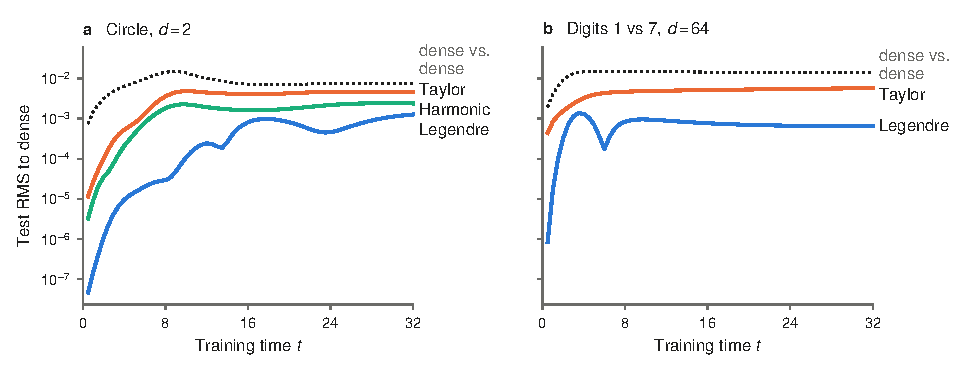
\includegraphics[width=\linewidth]{figures/exp_trajectory.pdf}
\caption{Error to the coupled width-4096 dense reference at every recorded
positive time, mean over three independent coupled references. The dotted
curve is the mean dense-versus-dense discrepancy. Models are those of
\Cref{tab:app-costs}; only declared query inputs are scored.}
\label{fig:app-trajectory}
\end{figure}

\begin{figure}[h]
\centering
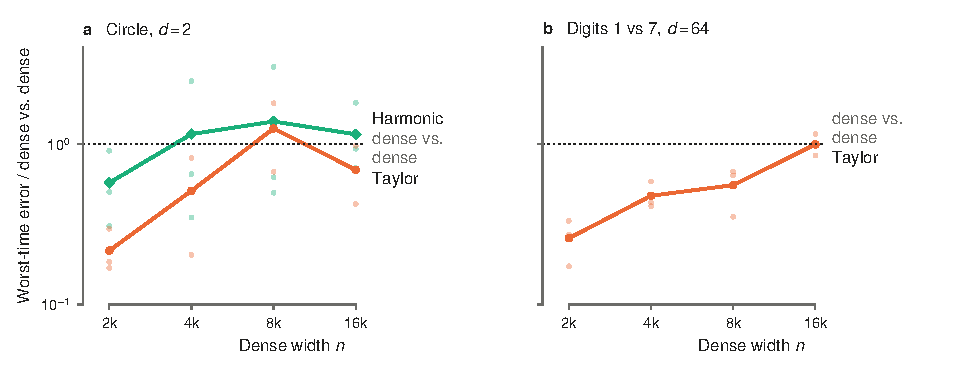
\includegraphics[width=\linewidth]{figures/exp_fixed_budget.pdf}
\caption{A fixed compact width of 512 as the dense reference widens. Each
point is the mean over three pairs of the ratio of the compression's
worst-time error to the dense pair's worst-time error; dots show the
individual pairs. All complete candidates are included, whether or not they
pass. Source settings may vary with dense width.}
\label{fig:app-fixed-budget}
\end{figure}

\begin{figure}[h]
\centering
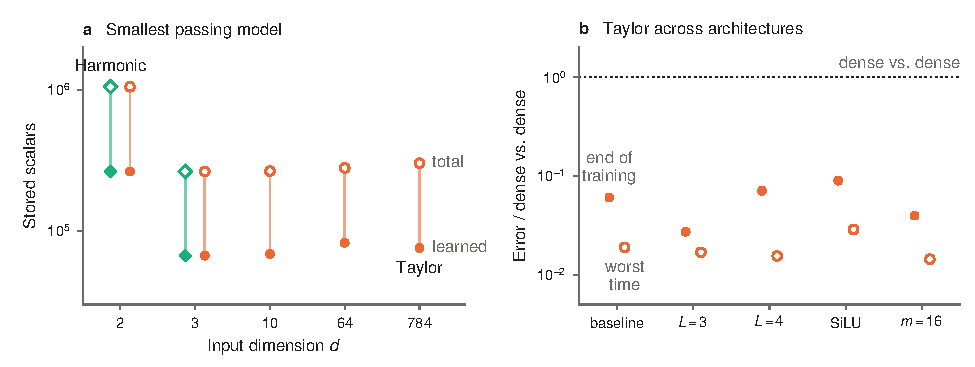
\includegraphics[width=\linewidth]{figures/exp_robustness.pdf}
\caption{(a) Smallest passing learned (filled) and total (hollow) storage
across input dimensions, using the worst-time criterion of
\Cref{fig:exp-storage}; at $d=784$ Taylor uses a fixed, counted projection
onto the panel span. (b) Taylor's endpoint and worst-time errors relative to
dense-versus-dense for five single-seed architecture variants with one
shared configuration: the two-layer baseline, three and four hidden layers,
SiLU activations, and sixteen training inputs.}
\label{fig:app-robustness}
\end{figure}

\begin{figure}[h]
\centering
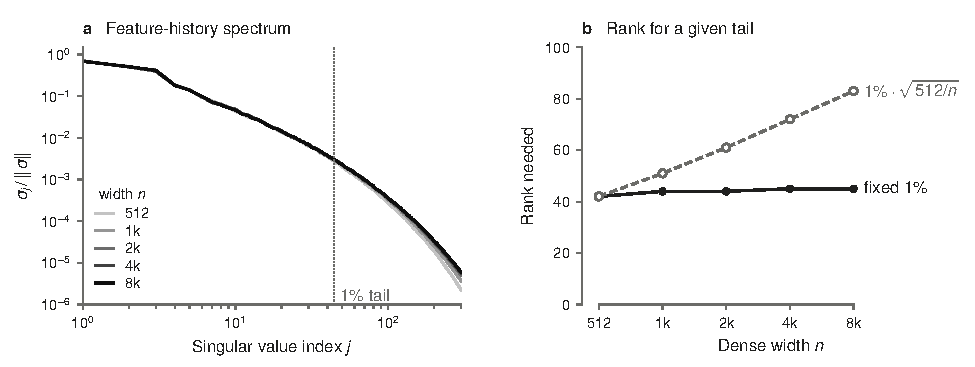
\includegraphics[width=\linewidth]{figures/exp_spectra.pdf}
\caption{(a) Normalized singular values of saved dense feature histories at
five widths. (b) Rank needed to leave a fixed $1\%$ relative tail (solid),
and a tail shrinking like $n^{-1/2}$ (dashed). The mandatory initial span is
additional. Single-seed reconstruction evidence, not a prediction-error
guarantee.}
\label{fig:app-spectra}
\end{figure}

\begin{figure}[h]
\centering
\begin{minipage}[t]{0.49\linewidth}
\centering
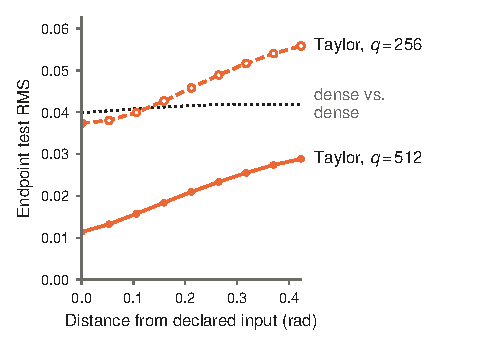
\includegraphics[width=\linewidth]{figures/exp_query_distance.pdf}
\end{minipage}\hfill
\begin{minipage}[t]{0.49\linewidth}
\centering
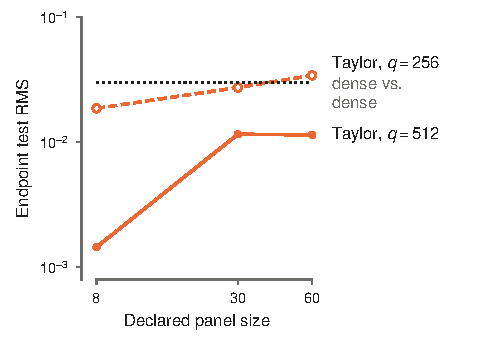
\includegraphics[width=\linewidth]{figures/exp_panel_size.pdf}
\end{minipage}
\caption{Scope of the declared panel. Left: Taylor's endpoint error along six
fixed geodesic paths leaving the declared inputs, for one seed in ambient
dimension 10 with a target depending on three coordinates. Right: panels of
8, 30 and 60 declared inputs at fixed source rank, all scored on the same
original queries. Labels of declared inputs are never used.}
\label{fig:app-panel}
\end{figure}

\begin{figure}[h]
\centering
\begin{minipage}[t]{0.49\linewidth}
\centering
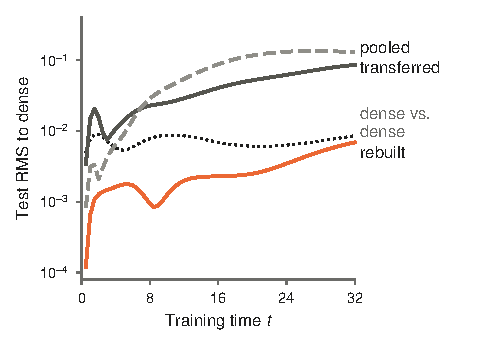
\includegraphics[width=\linewidth]{figures/exp_transfer.pdf}
\end{minipage}
\caption{Changing the labels after the sources are built. Sources rebuilt
for the new labels track the dense reference; sources transferred from the
old labels, or pooled across both, do not. The fixed-data theorem does not
promise label-independent sources.}
\label{fig:app-transfer}
\end{figure}

\begin{figure}[h]
\centering
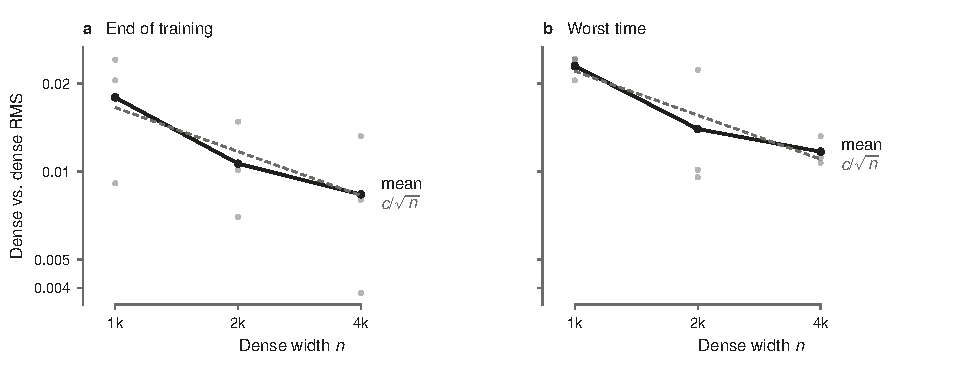
\includegraphics[width=\linewidth]{figures/exp_dense_pairs_sphere.pdf}
\par\medskip
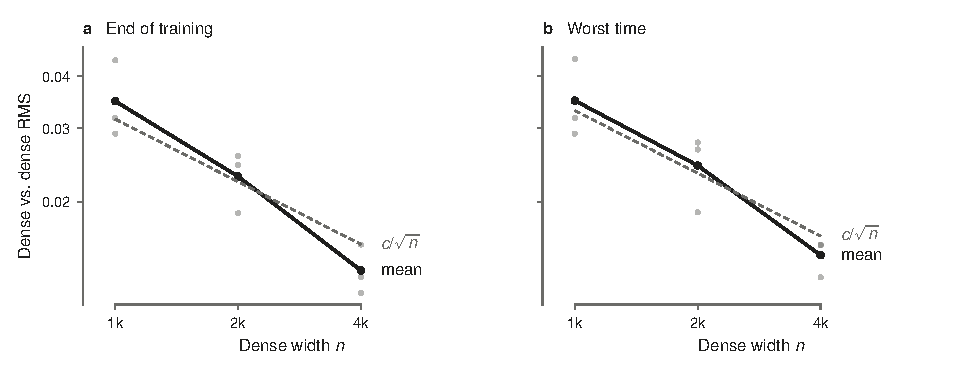
\includegraphics[width=\linewidth]{figures/exp_dense_pairs_mnist.pdf}
\caption{Independent dense discrepancy against width, at the end of
training and at the worst recorded time: sphere with $d=3$ (top) and raw
MNIST 1 versus 7 with $d=784$ (bottom). Three independent pairs per width;
dashed curves are descriptive $c/\sqrt n$ fits.}
\label{fig:app-dense-pairs}
\end{figure}
